%\chapter{Implementation Details}
 \chapter{Detalii de implementare}
\label{cap:implementare}


\section{Structura codului sursa}

Codul folosit pentru obținerea sistemului \textit{thesistitle} este împărțit în 3 proiecte separate: 
\begin{itemize}
	\item \textbf {Tor activity monitor} ce constituie logica necesară obținerii listei de adrese IP blocate de sistem. 
	\item \textbf{SQLi SVM} scopul acestuia fiind obținerea modelului de SVM folosit pentru prevenirea atacurilor de SQL injection. 
	\item \textbf{\thesistitle} reprezentând sistemul propus și încorporează rezultatele obținute de celelalte două proiecte. 
\end{itemize}

\begin{figure}[h]
	\centering
	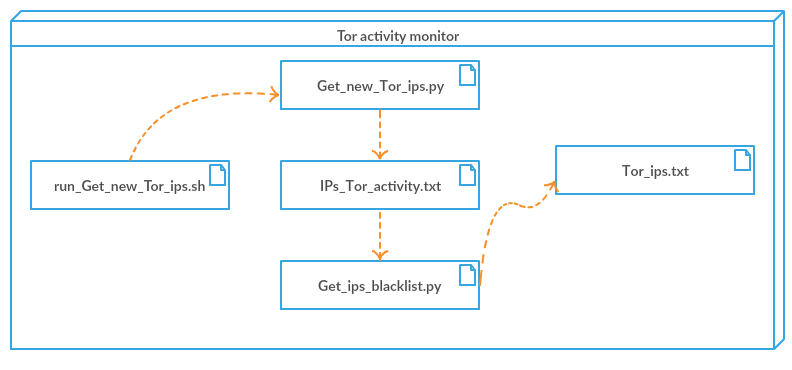
\includegraphics[width=0.8\textwidth]{tor_activity_monitor.png}
	\caption{Modulul pentru monitorizarea  activității rețelei Tor}
	\label{fig:tor_activity_monitor}
\end{figure}

Figura ~\ref{fig:tor_activity_monitor}  prezintă care sunt fișierele folosite pentru monitorizarea activității rețelei Tor și pentru obținerea listei cu adresele IP ce trebuie blocate de către sistem și relațiile dintre acestea. \\

\textbf{run\_Get\_new\_Tor\_ips.sh} este un fișier de bash ce are rolul de a rula Get\_new\_Tor\_ips.py. Fișierul este programat s a lanseze în execuție  Get\_new\_Tor\_ips.py  la ore fixe, acesta rulând încontinuu pe un sistem cu acces la internet neîntrerupt. Lansările în execuție au loc o data la 6 ore, respectiv la oră 12 am și pm și 6 am și pm. 

\textbf{Get\_new\_Tor\_ips.py}  are rolul de a documenta modificările de uptime din ultimele 6 ore ale nodurilor rețelei Tor. Datele sunt furnizate de pe pagina "Tor Network Status" \cite{tot_status} și pentru fiecare adresă IP prezentă în date, se verifică care este uptime-ul din ultimele 6 ore, informațiile acestea fiind stocate în  IPs\_Tor\_activity.txt.

\textbf{IPs\_Tor\_activity.txt}  are rolul de a stoca informațiile despre toate adresele IP utilizate de rețeaua tor din ultima luna. Acestea sunt salvate în liste, pentru fiecare adresă IP în parte o lista.  

\textbf{Get\_ips\_blacklist.py} are rolul de genera  fișierul  Tor\_ips.txt f olosit de către sistemul propus pentru blocarea adreselor IP. Acesta folosește datele din interiorul fișierului  IPs\_Tor\_activity.txt,  pentru a genera o lista cu toate adresele IP ce au un uptime total mai mare de 7 zile în ultimele 30 de zile. 

\textbf{Tor\_ips.txt}  reprezintă rezultatul proiectului. Acesta este alcătuit dintr-o lista formată din toate adresele IP ce vor fi blocate de sistemul propus în timpul rulării. 

\newpage

\begin{figure}[h]
	\centering
	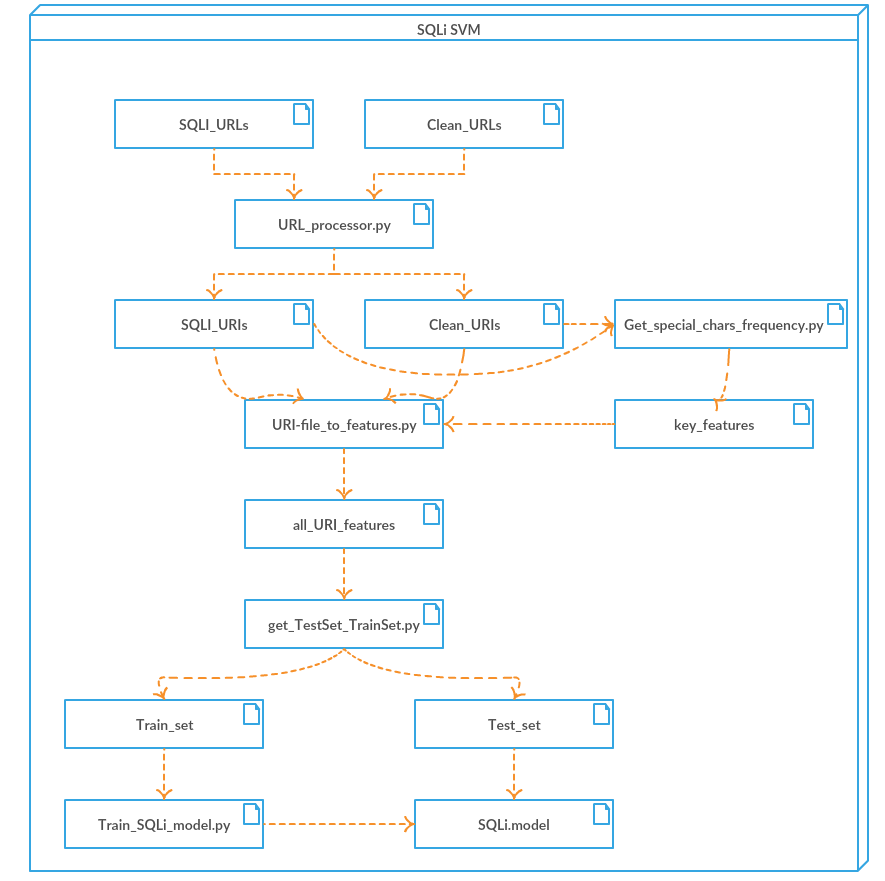
\includegraphics[width=0.8\textwidth]{sqli_svm.png}
	\caption{Modulul pentru prevenirea atacurilor SQL injection}
	\label{fig:sqli_svm}
\end{figure}
Figura ~\ref{fig:sqli_svm}  prezintă care sunt fișierele utilizate pentru procesarea datelor necesare în procesul de antrenare a modelului de SVM, până la obținerea modelului propriu-zis și care sunt relațiile dintre acestea. \\

\textbf{SQLI\_URLs}  reprezintă setul inițial de date "infected" folosite pentru identificarea atacurilor SQL injection. Acest set este constituit din URL-uri ce au fost identificate de un produs autorizat ca fiind tentative de SQL injection. 

\textbf{Clean\_URLs}  reprezintă setul inițial de date "clean" folosite pentru identificarea atacurilor SQL injection. Acest set este constituit din URL-uri ce au fost identificate de un produs autorizat ca fiind URL-uri curate. 

\textbf{URL\_processor.py}  primește ca input un fișier sau string și are rolul de a procesa URL-uri într-un format uniform(se elimină encodările) și specific pentru pașii următori. 

\textbf{SQLI\_URIs}  constituie nou lista rezultată din procesarea fișierului SQLI\_URLs de către URL\_processor.py.

\textbf{Clean\_URIs}  constituie noua lista rezultată din procesarea fișierului Clean\_URLs de către URL\_processor.py.

\textbf{Get\_secial\_chars\_frequency.py} are rolul de  a calcula frecvența de apariție a unor caractere speciale în cele două seturi de date și de a decide în funcție de frecvența lor de apariție, care din acestea sunt relevante în vederea alegerii trăsăturilor de clasificare. 

\textbf{key\_features} este  o listă alcătuită din toate cuvintele cheie a limbajului SQL, dar și din caracterele speciale utilizate în acesta și considerate ca fiind relevante în urma execuției scriptului  Get\_secial\_chars\_frequency.py.

\textbf{URI-file\_to\_features.py}  are rolul de a procesa cele două fișiere de date și pe baza trăsăturilor din  key\_features  să constituie un nou fișier ce conține pentru fiecare URL din cele două fișiere tipul acestuia și trăsăturile găsite în el, precum și frecvența lor.

\textbf{all\_URI\_features} este rezultatul rulării scriptului URI-file\_to\_features.py  și conține pentru fiecare URL din cele două fișiere de date, tipul acestuia și trăsăturile găsite în el, precum și frecvența lor, acestea fiind folosite pentru antrenarea și testarea modelului de SVM. 

\textbf{get\_TestSet\_TrainSet.py}  are rolul de a împarți datele prezente în  all\_URI\_features  în două seturi de proporție 70-30. Aceste două seturi fiind folosite pentru antrenarea și testarea modelului. 

\textbf{Train\_set} constituie 70\% din totalul de exemple acumulate pentru antrenarea modelului, doar acestea fiind de fapt folosite pentru antrenarea sa. 

\textbf{Test\_set} constituie 30\%  din exemplele acumulate, aceste date fiind folosite pentru testarea acurateții modelului după antrenare. 

\textbf{Train\_SQLi\_model.py} realizează obținerea modelului de SVM folosit de sistem pentru prevenirea atacurilor SQL injection. Pentru antrenare modelului este folosit setul de date din fișierul Test\_set și algoritmi puși la dispoziție de biblioteca open source libsvm  \cite{libsvm}.

\textbf{SQLi.model}  reprezintă rezultatul proiectului. Acesta este testat cu ajutorul setului de date din fișierul Test\_set și ulterior integrat în sistemul propus pentru a fi folosit pentru prevenirea atacurilor SQL injection. 

\newpage

\begin{figure}[h]
	\centering
	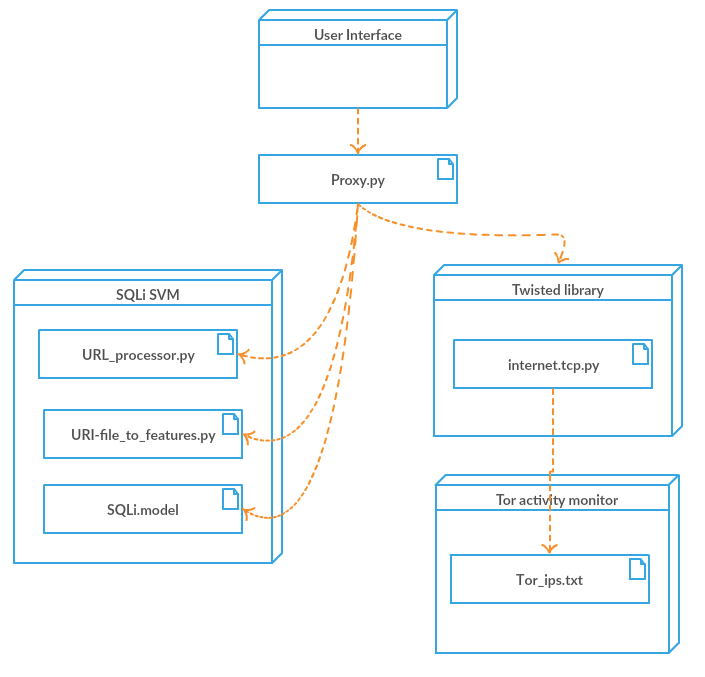
\includegraphics[width=0.8\textwidth]{source_code.png}
	\caption{ Interacțiunea dintre interfața grafică și celelalte module }
	\label{fig:source_code}
\end{figure}
Figura ~\ref{fig:source_code}  prezintă care sunt fișierele, specific fiecărui modul, care sunt accesate în mod direct de către interfață sau indirect de alte fișiere, în timpul rulării și relațiile dintre acestea. \\


\textbf{User Interface}  reprezintă întreaga componentă ce realizează interfața de utilizator cu toate fișierele necesare realizării ei incorporate în compoziția sa. Aceasta a fost realizată ca un proiect dezvoltat în .Net implicând multe fișiere cu scopul realizării elementelor grafice. Aceste elemente nu vor fi tratate în această secțiune. 

\textbf{Proxy.py}  reprezintă fișierul ce încorporează, respectiv leagă, tot codul ce constituie partea de "back end" a proiectului. În acest script de python se realizează instanțierea elementului de reverse proxy cu parametri de adrese IP și porturi aferente, precum și furnizarea metodelor de detecție componentei de reverse proxy. 

\textbf{Twisted library}  este o bibliotecă open source scrisă în Python, ce oferă suport pentru diferite protocoale (TCP, UDP, SSL/TLS). Biblioteca a fost folosită pentru partea de cod ce oferă implementarea unui reverse proxy. Mare parte din fișierele oferite de acesta bibliotecă au fost folosite fără a fi suprascrise sau a li se aduce modificări ulterioare, însă în vederea atingerii scopului propus, asupra unor fișiere sursă au fost aduse mici modificări (internet.tcp.py).

\textbf{internet.tcp.py} este scriptul din biblioteca twisted ce oferă suportul pentru protocolul TCP. Acest fișier a fost modificat pentru introducerea detecției împotriva utilizatorilor de Tor. Script-ul integrează lista realizată de proiectul "Tor activity monitor" pentru verificarea adresei utilizatorilor ce doresc să stabilească o conexiune TCP. 




\section{Algoritmi, metode si API-uri}

În acesta secțiune se urmărește descrierea codului sursă folosit la realizarea sistemului propus și explicarea amănunțită a codului/metodelor considerate mai relevante, precum și a principalelor api-uri utilizate în implementarea acestuia. Abordarea codului sursă se realizează conform sub-proiectelor prezentate în secțiunea anterioară (Tor activity monitor, AQLi SVM, Interfața utilizator). 

\subsection{Tor activity monitor}

Conform figurii ~\ref{fig:tor_activity_monitor},  acest proiect este realizat din 5 fișiere, acestea având o relație liniară între ele.

Fișierul ce începe ciclul de execuție,  run\_Get\_new\_Tor\_ips.sh, este un fișier de bash ce rulează în buclă infinită. Fișierul trebuie să ruleze pe un sistem ce este funcțional non-stop și cu acces nelimitat la internet. La ore fixe (12 am și pm și 6 am și pm), acesta lansează în execuție scriptul de python  Get\_new\_Tor\_ips.py.

Fișierul principal din acest proiect îl reprezintă  Get\_new\_Tor\_ips.py.  Acesta descărcă pagina "Tor Network Status" \cite{tot_status}  și procesează datele de pe acestea, introducând în fișierul IPs\_Tor\_ activity.txt  informații referitoare la adresele IP găsite pe pagină și uptime-ul lor din ultimele 6 ore. Procesarea adreselor IP și extragerea valorii lor de uptime se poate observa în următoarele două secvențe de cod. 

\lstset{language=python,frame=single, showstringspaces=false}
\begin{lstlisting}
time_up = row.findAll('td')[4].contents[0]
ip = row.findAll('td', attrs={'class':'iT'})[0].findAll('a',
 attrs={'class':'who'})[0].contents[0]


\end{lstlisting}

Pentru prelucrarea conținutului paginii, acesta a fost download-at în memoria programului, iar codul HTML rezultant a fost prelucrat cu ajutorul bibliotecii de python open source, BeautifulSoup. Codul de mai sus reprezintă extragerea valori de timp (uptime) și adresa IP căreia aceasta corespunde. Variabila "row" fiind un element din obiectul iterabil rezultat din inițializarea bibliotecii BeautifulSoup cu codul HTML al paginii. 

\lstset{language=python,frame=single, showstringspaces=false}
\begin{lstlisting}
days = time_up.split()[1]
if days == 'd':
    hours = 6
else:
    hours = int(time_up.split()[0])
    if hours > 6:
        hours = 6

\end{lstlisting}

În secvența de mai sus de cod, este identificata valoarea corectă de uptime din ultimele 6 ore. Pentru cazul în care valoare de uptime este sub formă de zile sau aceasta este mai mare de 6 ore, ea se setează pe 6 ore, întrucât nu ne interesează decât activitatea din ultimele 6 ore. 
\begin{lstlisting}
from bs4 import BeautifulSoup
from urllib.request import urlopen

pagesource = urlopen(page)
soup = BeautifulSoup(pagesource.read())
table = soup.findAll('table', attrs={'class': 'displayTable'})
\end{lstlisting}

Pentru procesarea  conținutului unei pagini web("Tor Network Status" \cite{tot_status}) s-au folosit bibliotecile de python, open source, urllib și BeautifulSoup \cite{btf_soup}.  Biblioteca urllib oferă funcții și clase ce pot fi folosite pentru deschiderea de URL-uri (urlopen). Funcția folosită în codul de mai sus primește ca parametru "page" adresa sub formă de string a paginii ce se dorește a fi citită. Biblioteca BeautifulSoup este o bibliotecă de python folosită pentru extragerea de date din fișiere de HTML sau XML. Acesta este inițializată cu un document HTML/XML și că rezultat oferă un obiect ce permite navigarea prin codul sursă asemeni unei structuri de date imbricate. Astfel, spre exemplu, pentru identificarea structurii corespunzătoare tabelei de adrese IP din codul sursă al paginii s-a folosit o singură linie de cod, în care s-au specificat numele și atributele specifice acesteia. 

Rezultatele rulării fișierului  Get\_new\_Tor\_ips.py sunt  actualizate în  IPs\_Tor\_activity.txt.  Acest fișier este de fapt un json în care se realizează dump la noul dicționar obținut de   Get\_new\_Tor\_ips.py.  Dicționarul este constituit din adresa IP ca și cheie și o listă .Structura acestor liste este realizată dintr-o serie de numere între 0 și 6 ce reprezintă timpul total de uptime corespunzător sfertului respectiv de zi. Dimensiunea acestei liste este fixată la 30 (zile) *4 (sferturi de zi), pe măsură ce un element nou este adăugat, primul element din lista fiind scos. 

Următorul pas este filtrarea tuturor adreselor IP ce au un uptime mai mare de 7 zile. Acest lucru este realizat de scriptul  Get\_ips\_blacklist.py, iar rezultatele sunt stocate în Tor\_ips.txt, o adresă IP pe linie. 

\subsection{SQLi SVM}
Desfășurarea proiectului începe de la cele două fișiere SQLi\_URLs si Clean\_URLs.  În aceste două fișiere se află URL-uri complete din categoria conformă cu numele fiecărui fișier. Aceste fișiere sunt procesate de scriptul  URI\_processor.py  care are rolul de a uniformiza datele în aceeași encodare. Următoarea bucată de cod prezintă secvența ce transformă valorile hexa dintr-un URI în caractere și modul în care erorile de encodare sunt tratate (sunt afișate pentru a fi tratate manual de către programator): 

\lstset{language=python,frame=single, showstringspaces=false}
\begin{lstlisting}
for index, sub_uri in enumerate(uri.split('%')):
    if sub_uri:
        if index == 0:
            new_uri = sub_uri
            continue
        try:
            hex_val = bytearray.fromhex(sub_uri[:2]).decode()
        except UnicodeDecodeError:
            print(uri + ' --- ' + sub_uri[:2])
            return ''
        new_uri += hex_val + sub_uri[2:]
\end{lstlisting}

Întrucât într-un URL caracterul '\%' nu poate să apăra decât dacă acesta este encodat ('\%25'- valoarea pentru encodarea caracterului '\%'), identificarea tuturor caracterelor encodate a fost făcută prin identificarea tuturor caracterelor de tipul '\%' în URI. În cazul în care un astfel de caracter este găsit, se încearcă conversia următoarelor două caractere (așteptându-se, conform convenției, să fie cifre sau litere de la A la F), din valoarea în hexa corespunzătoare unui anumit caracter în caracterul în sine. 

  
În urma procesării datelor, rezultă cele două fișiere  SQLi\_URIs si Clean\_URIs,  acestea având același conținut ca cele anterioare însă în aceeași encodare. În urma obținerii acestor două fișiere, a fost realizată completarea listei de trăsături (lista inițială este constituită din toate cuvintele cheie a limbajului SQL) cu caracterele speciale întâlnite în acest limbaj. Scriptul  Get\_secial\_chars\_frequency.py  are rolul de a determina frecvența de apariție a fiecărui caracter special în cele două seturi de date, iar pe baza unei observații umane, a fost realizată determinarea caracterelor ce constituie trăsături rentabile. Următoarea bucată de cod este din scriptul Get\_secial\_chars\_frequency.py  și realizează numărarea URI-urilor(pentru comparare) din setul de date și frecvența caracterelor speciale("dict" este un dicționar cu cheile fiind caracterele speciale utilizate în limbaj): 
\lstset{language=python,frame=single, showstringspaces=false}
\begin{lstlisting}
with open(args.f, 'r') as fd:
    for lines in fd.readlines():
        lines_nr += 1
        line = lines.strip()
        for keys in dict:
            if keys in line:
                dict[keys] += 1
                
\end{lstlisting}

Pentru identificarea caracterelor relevante din limbajul SQL în comparație cu cele folosite într-un URL obișnuit, s-a ales numărarea frecvenței de apariție a acestora în URL-uri normale, dar și în URL-uri ce conțin atacuri de SQL injection. Numărarea se face alternativ, rezultatele fiind furnizate că două seturi de date separate, bucata anterioară de cod reprezentând procesul doar pentru una dintre cele două categorii. Dicționarul referit în cod este alcătuit dintr-un dicționar ce are că și chei valoarea caracterelor speciale căutate, iar ca valoare, acestea sunt inițializate pe zero pentru a fi incrementate o data cu numărul de apariții ale caracterelor căutate. Pentru uniformizarea setului de date, întrucât distribuția acestor caractere nu este tot timpul uniformă, se ține cont și de numărul de linii (pe fiecare linie se află un URI distinct) în care au fost identificate frecvențele lor de apariție. 

După determinarea caracterelor relevante, acestea au fost completate manual în fișierul key\_features, fișier ce însumează toate trăsăturile ce sunt folosite în antrenarea modelului (fiecare linie conține o trăsătură, numărul liniei fiind și indicele de referință a trăsăturii). 

Pentru obținerea datelor într-un format ce poate fi procesat de biblioteca libsvm \cite{libsvm} a fost necesară transformarea acestora într-un anumit format: 

\begin{lstlisting}
+1 23:1 37:4 103:2
-1 54:1 77:1
\end{lstlisting}

Conversia URI-urilor în formatul de mai sus este realizată de scriptul  URI-file\_to\_features.py.  Formatul de mai sus este reprezentarea fiecărui URL în funcție de tipul acestuia și indicele trăsăturii găsite în interiorul sau precum și frecvența de apariție a acestora (tip trăsătură : trăsătură : frecvență). Următoarele bucăți de cod sunt extrasă din fișieru l URI-file\_to\_features.py  și realizează conversia unui URI în echivalentul sau în trăsături: 

\begin{lstlisting}
if keys in uri:
 if keywords_list.index(keys) > 184:
  keywords[keys] = uri.count(keys)
  if not uri.count(keys) == 0:
    ok = True
\end{lstlisting}

În lista cu trăsături, primele 184 de poziții corespund cuvintelor cheie ale limbajului SQL, următoarele 8 poziții aparținând trăsăturilor de tipul caracter special (determinate la pasul anterior de script-ul "Get\_special\_chars\_frequency.py"). În cazul în care o astfel de trăsătură este găsită într-un URI, pur și simplu se găsește numărul total de apariții a caracterului respectiv în URI. 


\begin{lstlisting}
sub_uri = uri.split(keys)
for index, ele in enumerate(sub_uri):
  if index + 1 < len(sub_uri):
    if ele and sub_uri[index + 1] and not ele[-1].isalpha()
     and not sub_uri[index+1][0].isalpha():
      keywords_aux[keys] += 1
  elif not ele and sub_uri[index - 1]:
      keywords_aux[keys] += 1
\end{lstlisting}

Pentru trăsăturile de pe primele 184 de poziții, adică cuvintele cheie ale limbajului SQL, s-a abordat o logică mai complexă de procesare. O data ce un cuvânt este găsit într-un URI, pentru fiecare apariție a acestui cuvânt se verifică ca primul caracter anterior cuvântului și primul următor cuvântului să nu fie literă, astfel eliminându-se cazurile în care unele cuvinte sunt incluse în altele (ex:  \textbf{all} și de\textbf{all}ocate).

În urma procesării fișierelor de date, rezultă un fișier  (all\_URI\_features)  ce însumează toate datele utilizate în antrenarea modelului(exemple atât pozitive cât și negative), însă sub formă prezentată anterior (tip trăsătură :  trăsătură : frecvență). Acest fișier este împărțit în două fișiere cu proporția  de 70\% pentru Train\_set și 30\% Tes\_set de scriptul get\_Trainset\_Testset.py.  cu scopul de a obține un grup de date atât pentru antrenarea modelului cât și pentru testarea ulterioară a acestuia. 

Pentru antrenarea modelului, s-a folosit biblioteca open sourece libsvm. Această bibliotecă furnizează fișierele necesare antrenării modelului de svm și de prezicere a unui rezultat pe un model existent. Apelul către executabilul "svm-train.exe" se face prin intermediul scriptului de python  Train\_SQLi\_model.py.
Executabilul de windows furnizat de biblioteca libsvm poate fi apelat conform exemplului următor: 

\begin{lstlisting} 
svm-train.exe [options] training_set_file [model_file]
\end{lstlisting}

\subsection{Interfață utilizator}

 Componenta de interfață reprezintă atât proiectul în .net în care a fost realizată interfață sistemului, dar și fișierele/script-urile ce au rolul de a interconecta rezultatele celor două proiecte anterioare cu acesta. 

Scriptul Proxy.py încapsulează toate elementele, din partea de back end, a proiectului propus. Acesta de asemenea furnizează ca output într-un format specific (format ce este cunoscut și interpretat de interfața grafică) toate evenimentele ce apar în timpiul rulării sistemului. În acest script se realizează instanțierea elementului de reverse proxy cu parametri de adrese IP și porturi aferente, precum și furnizarea metodelor de detecție componenței de reverse proxy. Inițializarea elementului de reverse proxy se realizează cu ajutorul codului oferit de biblioteca twisted. Acest cod este prezentat în "Anexa A" a acestei lucrări. 

În următoarele imagini sunt prezentate posibilele pagini ale interfeței utilizator precum și o scurtă descriere ce ilustrează funcționalitățile oferite de paginile respective pentru utilizator. 

 \newpage
\begin{figure}[h]
	\centering
	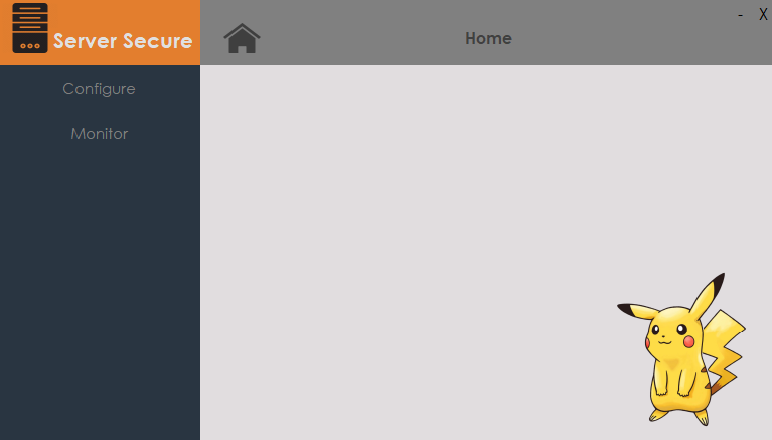
\includegraphics[width=0.6\textwidth]{ui_home.png}
	\caption{Meniul "Home" in interfata grafica}
	\label{fig:ui_home}
\end{figure}
Figura ~\ref{fig:ui_home}  prezintă design-ul paginii de "Home" din interfața grafică pusă la dispoziție utilizatorilor sistemului. Acesta pagină este afișată la lansarea în execuție a aplicație, dar poate fi accesata de către utilizator și prin apăsarea butonului în formă de "căsuță" din dreapta logoului aplicației. \\

\begin{figure}[h]
	\centering
	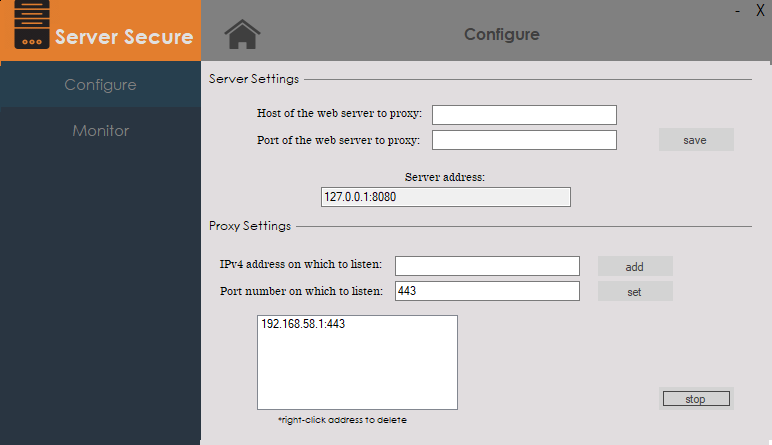
\includegraphics[width=0.7\textwidth]{ui_configure.png}
	\caption{Meniul "Configure" in interfața grafica}
	\label{fig:ui_configure}
\end{figure}

Figura ~\ref{fig:ui_configure}  prezintă design-ul paginii de "Configure" din interfața grafică, în care utilizatorul sistemului poate să seteze interfețele și porturile care vor fi tratate în timpul rulării. Partea superioară a meniului reprezintă setările aferente părții de server, precum sugerează și eticheta din stânga sus "Server Settings". În partea inferioară se pot seta detaliile interfețelor ce se pot conecta la server-ul setat mai sus (aceste interfețe pot fi multiple).  \\
\newpage
\begin{figure}[h]
	\centering
	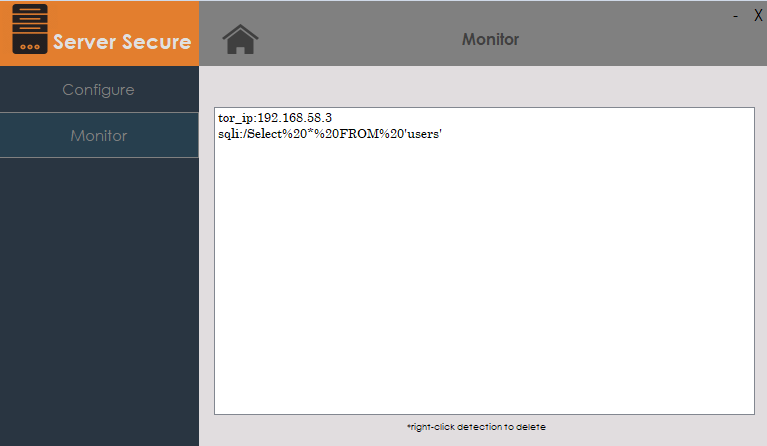
\includegraphics[width=0.8\textwidth]{ui_monitor.png}
	\caption{Meniul "Monitor" in interfața grafica}
	\label{fig:ui_monitor}
\end{figure}
Figura ~\ref{fig:ui_monitor}  prezintă design-ul paginii de "Monitor" din interfața grafică, în care utilizatorul poate să urmărească activitatea sistemului în timpul rulării. În această fereastră apar evenimentele apărute în timpul rulării aplicației, evenimente ce sunt sub formă de detecții. \\

\begin{figure}[h]
	\centering
	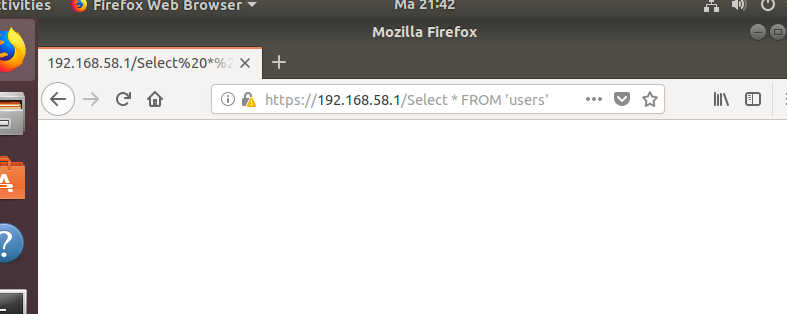
\includegraphics[width=0.9\textwidth]{sqli_respons.png}
	\caption{Raspunsul pentru SQL injection URL}
	\label{fig:sqli_respons}
\end{figure}

Figura ~\ref{fig:sqli_respons}  prezintă cum arată răspunsul primit de la server de către un utilizator după trimiterea unui request către server, cu intenția de a realiza un atac de tipul SQL injection. Utilizatorului i se returnează o pagină goală. \\

\begin{figure}[h]
	\centering
	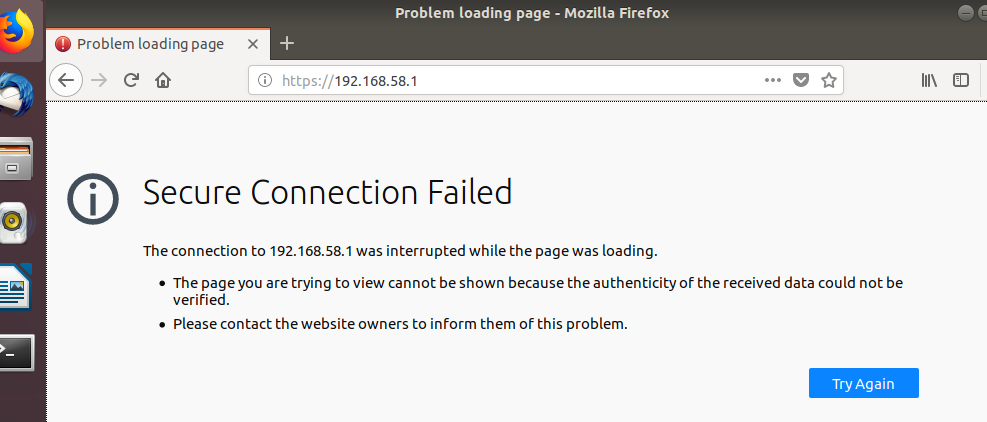
\includegraphics[width=0.8\textwidth]{tor_respons.png}
	\caption{Principalele module ale sistemului propus}
	\label{fig:tor_respons}
\end{figure}
Figura ~\ref{fig:tor_respons}  prezintă cum arată răspunsul primit de la server de către un utilizator al rețelei Tor ce intenționează să se conecteze la acesta. Acestor utilizatori li se refuză conexiunea.  \\


%
%
%Conține detalii de implementare: 
%\begin{itemize}
%  \item organizarea codului sursă, organizarea logică a codului (module, ierarhii de clase)
%  \item descrierea claselor, funcțiilor, API-urilor importante ale aplicației
%  \item descrierea la nivel de implementare a algoritmilor principali
%  \item descrierea părților mai dificile
%  \item alte detalii de implementare relevante, specifice fiecărei aplicații
%\end{itemize}
%
%Descrierea implementării trebuie să reflecte modul în care ea corespunde (se mapează) design-ului. 
%
%Nu se vor da detalii irelevante. Descrierea codului trebuie gândită ca un ghid de parcurgere a codului sursă de către cineva care vrea să continue proiectul vostru. 
%
%Exemplu de cod:
%\lstset{language=C,frame=single, showstringspaces=false}
%\begin{lstlisting}
%# include <stdio.h>
%  
%int main (int argc, char **argv)
%{
%  int i;
%    
%  for (i=0; i<argc; i++)
%    printf("argv[%d] = %s\n", i, argv[i]);
%    
%  return 0;
%}
%\end{lstlisting}